% --------------------------------------------------------------------------- %
% A0 paper poster for MetrumRG						   %
% --------------------------------------------------------------------------- %
% Created with Brian Amberg's LaTeX Poster Template. 					     %
% --------------------------------------------------------------------------- %

\documentclass[a0paper,portrait]{baposter}

\usepackage{relsize}		% For \smaller
\usepackage{url}			% For \url
\usepackage{epstopdf}	% Included EPS files automatically converted to PDF to include with pdflatex
\usepackage{graphicx}
\usepackage{setspace}
\spacing{1}

\usepackage[bitstream-charter]{mathdesign}
\usepackage[T1]{fontenc}

% Deprecating osfigures option; use oldstyle instead; 2020-09-10
\usepackage[defaultsans,oldstyle,scale=0.95]{opensans}

%%% Global Settings %%%%%%%%%%%%%%%%%%%%%%%%%%%%%%%%%%%%%%%%%%%%%%%%%%%%%%%%%%%

\graphicspath{{pix/}}	% Root directory of the pictures 
\tracingstats=2			% Enabled LaTeX logging with conditionals

%%% Color Definitions %%%%%%%%%%%%%%%%%%%%%%%%%%%%%%%%%%%%%%%%%%%%%%%%%%%%%%%%%

\definecolor{bordercol}{RGB}{40,40,40}
\definecolor{headercol1}{RGB}{186,215,230}
\definecolor{headercol2}{RGB}{80,80,80}
\definecolor{headerfontcol}{RGB}{0,0,0}
\definecolor{boxcolor}{RGB}{186,215,230}
\definecolor{metgreen}{rgb}{0,0.555,0}
\definecolor{lightergreen}{rgb}{.8,1,0.85}
\definecolor{lightergray}{RGB}{225,225,225}
\definecolor{darkteal}{RGB}{41, 127, 157}
\definecolor{tealdark}{RGB}{41, 104, 157}
\definecolor{black}{RGB}{0,0,0}

% PLEASE MODIFY COLOR SCHEME HERE IF NEEDED
\colorlet{titlefgcol}{black}
\colorlet{headerbgcol}{darkteal}
\colorlet{headerfgcol}{white}
\colorlet{bordercol}{lightergray}
\newcommand{\headershade}{none}

%%%%%%%%%%%%%%%%%%%%%%%%%%%%%%%%%%%%%%%%%%%%%%%%%%%%%%%%%%%%%%%%%%%%%%%%%%%%%%%%
%%% Utility functions %%%%%%%%%%%%%%%%%%%%%%%%%%%%%%%%%%%%%%%%%%%%%%%%%%%%%%%%%%

%%% Save space in lists. Use this after the opening of the list %%%%%%%%%%%%%%%%
\newcommand{\compresslist}{
	\setlength{\itemsep}{1pt}
	\setlength{\parskip}{0pt}
	\setlength{\parsep}{0pt}
}

%%%%%%%%%%%%%%%%%%%%%%%%%%%%%%%%%%%%%%%%%%%%%%%%%%%%%%%%%%%%%%%%%%%%%%%%%%%%%%%
%%% Document Start %%%%%%%%%%%%%%%%%%%%%%%%%%%%%%%%%%%%%%%%%%%%%%%%%%%%%%%%%%%%
%%%%%%%%%%%%%%%%%%%%%%%%%%%%%%%%%%%%%%%%%%%%%%%%%%%%%%%%%%%%%%%%%%%%%%%%%%%%%%%

\begin{document}
\typeout{Poster rendering started}

%%% Setting Background Image %%%%%%%%%%%%%%%%%%%%%%%%%%%%%%%%%%%%%%%%%%%%%%%%%%
\background{
%	\begin{tikzpicture}[remember picture,overlay]%
%	\draw (current page.north west)+(-2em,2em) node[anchor=north west]
%	{\includegraphics[height=1.1\textheight]{background}};
%	\end{tikzpicture}
}

%%% General Poster Settings %%%%%%%%%%%%%%%%%%%%%%%%%%%%%%%%%%%%%%%%%%%%%%%%%%%
%%%%%% Eye Catcher, Title, Authors and University Images %%%%%%%%%%%%%%%%%%%%%%
\begin{poster}{
	grid=false,
	% Option is left on true though the eyecatcher is not used. The reason is
	% that we have a bit nicer looking title and author formatting in the headercol
	% this way
	% columns = 4,
	eyecatcher=false, 
	borderColor=bordercol,
	headerColorOne=headerbgcol,
	headerColorTwo=headerbgcol,
	headerFontColor=headerfgcol,
	% Only simple background color used, no shading, so boxColorTwo isn't necessary
	boxColorOne=white,
	headershape=rectangle,
	headerfont=\Large\bf\textsf,
	textborder=rectangle,
	background=user,
	headerborder=open,
  boxshade=none, 
  headershade=plain,
  headerheight=0.1\textheight %% CHANGE THIS TO INCREASE ROOM FOR LONG TITLE
}
%%% Eye Cacther %%%%%%%%%%%%%%%%%%%%%%%%%%%%%%%%%%%%%%%%%%%%%%%%%%%%%%%%%%%%%%%
{
%	Eye Catcher, empty if option eyecatcher=false - unused
}
%%% Title %%%%%%%%%%%%%%%%%%%%%%%%%%%%%%%%%%%%%%%%%%%%%%%%%%%%%%%%%%%%%%%%%%%%%
{
	\textbf{\textsf{\color{titlefgcol}{
	\huge
	  A multi-organ integrated QSP model for hematopoietic stem cell differentiation to predict the immune cell reconstitution in ex-vivo gene therapy
	 }}}\vspace{.5em}
}
%%% Authors %%%%%%%%%%%%%%%%%%%%%%%%%%%%%%%%%%%%%%%%%%%%%%%%%%%%%%%%%%%%%%%%%%%
{
\normalsize
	Yuezhe Li$^1$, Eric Jordie$^1$, Tim Knab$^1$\\
	{\smaller
	  $^1$\textit{Metrum Research Group}
	}
}
%%% Logo %%%%%%%%%%%%%%%%%%%%%%%%%%%%%%%%%%%%%%%%%%%%%%%%%%%%%%%%%%%%%%%%%%%%%%
{
% The logos are compressed a bit into a simple box to make them smaller on the result
% (Wasn't able to find any bigger of them.)
%\setlength\fboxsep{5pt}
%\setlength\fboxrule{0.5pt}
%	\fbox{
		\begin{minipage}{16em}
			\begin{center}
			
\includegraphics[width=14em]{newlogo} 
			\end{center}
		\end{minipage}
%	}
}
%%%%%%%%%%%%%%%%%%%%%%%%%%%%%%%%%%%%%%%%%%%%%%%%%%%%%%%%%%%%%%%%%%%%%%%%%%%%%%%%
%%%%%%%%%%%%%%%%%%%%%%%%%%%%%%%%%%%%%%%%%%%%%%%%%%%%%%%%%%%%%%%%%%%%%%%%%%%%%%%%


\headerbox{Abstract}{name=abstract,column=0,row=0}{
\footnotesize

The differentiation of mammalian hematopoietic stem cells (HSCs) is complex and multi-scale, providing an opportunity for mathematical modeling and simulation to aid in mechanistic understanding and ultimately inform drug development efforts. Historically, mathematical models have been developed that were focused on the development of a subset of cells, but mathematical models that encompass the overall cellular system’s complexity are rarely available. Here, we develop an integrated quantitative systems pharmacology (QSP) model that characterizes multi-organ recapitulation of HSC differentiation by integrating literature models and adding novel features. The result is a more comprehensive representation of mammalian hematopoietic stem cell development. We demonstrate our integrated model can accurately capture the reconstitution of RBCs, B cells, and T cells following HSC transplant in mice. Moreover, the humanized model successfully predicted the reconstitution of granulocytes and lymphocytes  in patients with adenosine deaminase‐deficient severe combined immunodeficiency (ADA-SCID) who underwent ex-vivo gene therapy. 


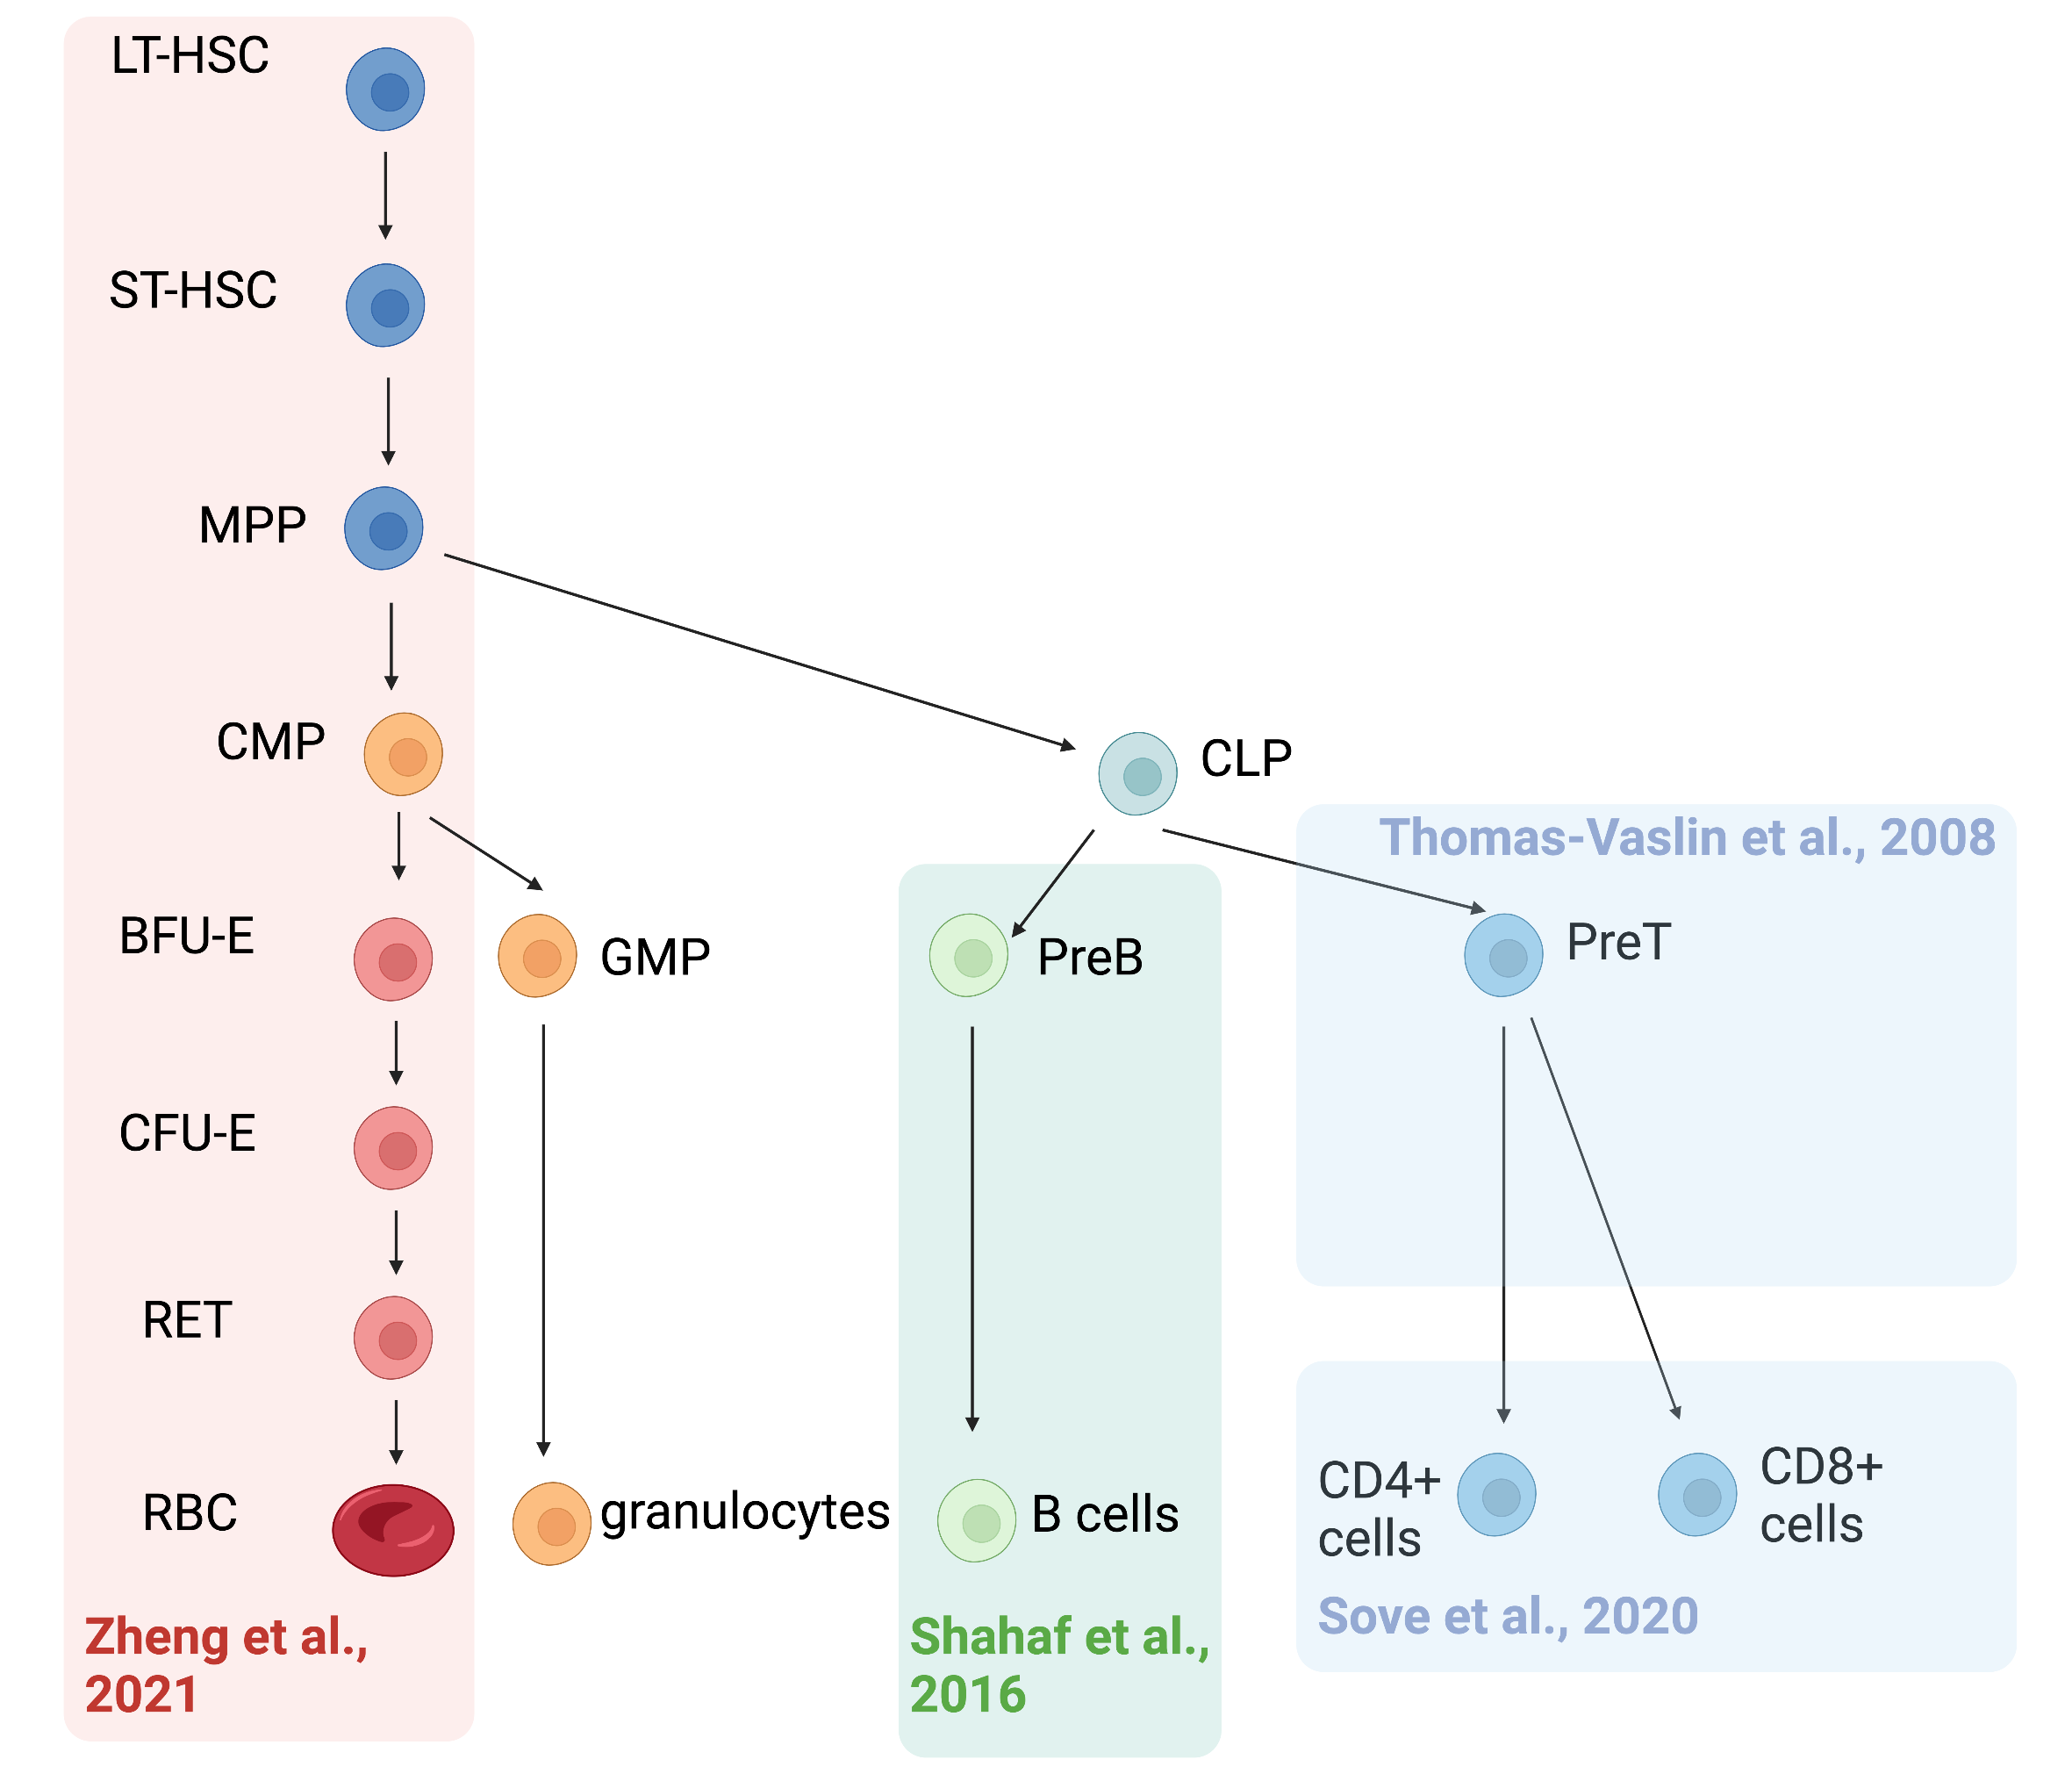
\includegraphics[width= 0.8 \textwidth]{../img/Diagram_integration}

}
%%%%%%%%%%%%%%%%%%%%%%%%%%%%%%%%%%%%%%%%%%%%%%%%%%%%%%%%%%%%%%%%%%%%%%%%%%%%%%%%

\headerbox{Methods}{name=methods,column=0,below=abstract}{
\footnotesize

We developed an integrated model that depicts the differentiation of hematopoietic stem cells (HSCs) into erythrocytes, lymphocytes, and granulocytes. The model was built incrementally by incorporating novel physiological-based features from literature while integrating published models:
\begin{itemize}
%\setlength{\itemindent}{-2em}
  \item human HSC differentiation into red blood cells (RBCs) [1]
  \item mouse B cell development [2]
  \item mouse T cell development [3]
  \item human naive T cell dynamics model [4]
\end{itemize}

The model was developed in 4 steps: 
\begin{itemize}
  \item Implement an existing human HSC -> RBC differentiation model in [1]
  \item Scale the HSC -> RBC differentiation model from human to mouse
  \item Integrate T cells development model from [3], B cells development model from [2], and HSC -> granulocyte differentiation model into the mouse differentiation model 
  \item Scale the integrated mouse HSC differentiation model to human.
\end{itemize}

Further parameter tunings were carried out using steady state data (e.g. blood cell count) in mouse and in human. The integrated models for mouse and human were validated using cell reconstitution in peripheral blood after stem cell transplant/ ex-vivo gene therapy. 

}

%%%%%%%%%%%%%%%%%%%%%%%%%%%%%%%%%%%%%%%%%%%%%%%%%%%%%%%%%%%%%%%%%%%%%%%%%%%%%%%%

\headerbox{References}{name=references,column=0,below=methods}{
\scriptsize	
[1] Zheng, Bo, et al. "A systems pharmacology model for gene therapy in sickle cell disease." CPT: Pharmacometrics \& Systems Pharmacology 10.7 (2021): 696-708.
[2] Shahaf, Gitit, et al. "B cell development in the bone marrow is regulated by homeostatic feedback exerted by mature B cells." Frontiers in immunology 7 (2016): 77.
[3] Thomas-Vaslin, Veronique, et al. "Comprehensive assessment and mathematical modeling of T cell population dynamics and homeostasis." The Journal of Immunology 180.4 (2008): 2240-2250.
[4] Sové, Richard J., et al. "QSP‐IO: a quantitative systems pharmacology toolbox for mechanistic multiscale modeling for Immuno‐oncology applications." CPT: pharmacometrics \& systems pharmacology 9.9 (2020): 484-497.
}
%%%%%%%%%%%%%%%%%%%%%%%%%%%%%%%%%%%%%%%%%%%%%%%%%%%%%%%%%%%%%%%%%%%%%%%%%%%%%%%%
%%%%%%%%%%%%%%%%%%%%%%%%%%%%%%%%%%%%%%%%%%%%%%%%%%%%%%%%%%%%%%%%%%%%%%%%%%%%%%%%


\headerbox{Results}{name=results,span=2,column=1,row=0}{
\footnotesize

The integrated HSC differentiation model for mouse can be summarized by the figure follow. 
Briefly, the long-term hematopoietic stem cells (LT-HSC) is capable of self-renewal and can differentiate to be short-term hematopoietic stem cells (ST-HSC). 
ST-HSC can differentiate to be multipottrnt ptogrnitor cells (MPP). 
MPP can differentiate to be common myeloid progenitor (CMP) or common lymphoid progenitor (CLP). 
CMP can differentitiate to be burst forming unit-erythroid (BFU-E) and granulocyte-monocyte progenitors (GMP). 
BFU-E can differentiate to be colony forming unit-erythroid (CFU-E), then reticulocytes (RET) and red blood cells (RBC). Furthermore, hemoglobin (Hb) can be synthesized in RETs and RBCs, and the oxygen level in blood imposes a negative feedback on CFU-E amplification. 
The erythrocytes differentiation model was taken from [1]  and scaled from human to mouse by reparameterize of mean residence time and amplification number is based on rates and observations provided in Busch et al., Nature. 2015, Putten and Croon, Blood. 1958, Ney Curr Opin Hematol. 2011, and Palis, Front Physio. 2014.  
CLP can further differentiate into B cells and T cells in bone marrow, spleen (diagram in middle panel, model obtained from [2]) and thymus (diagram in right panel, model obtained from [3]). 
GMP can further differentiate to be granulocytes (GM). 


\begin{minipage}[b]{0.55\linewidth}
\centering
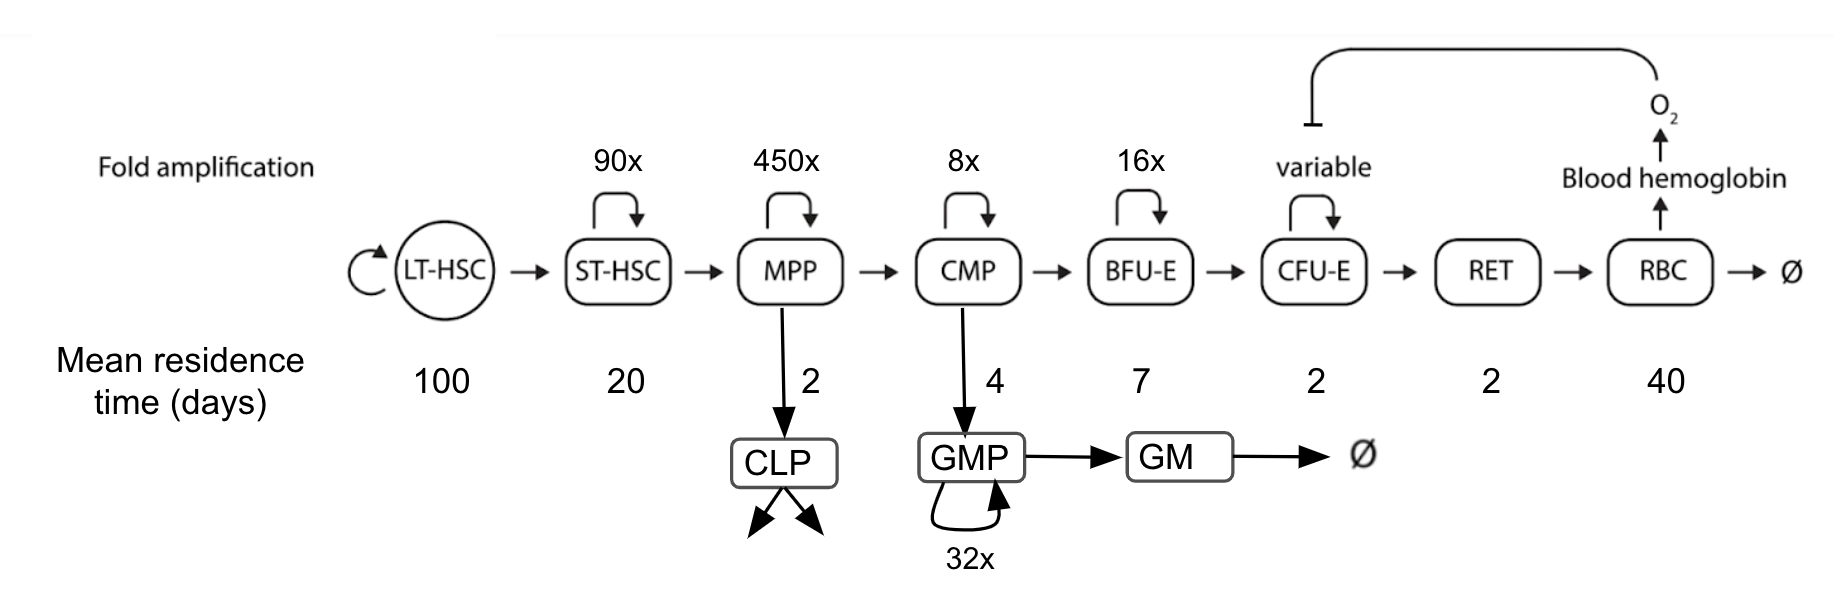
\includegraphics[width=\textwidth]{../img/mouse_full_model.png}
\end{minipage}
\hspace{0.5cm}
\begin{minipage}[b]{0.4\linewidth}
\centering
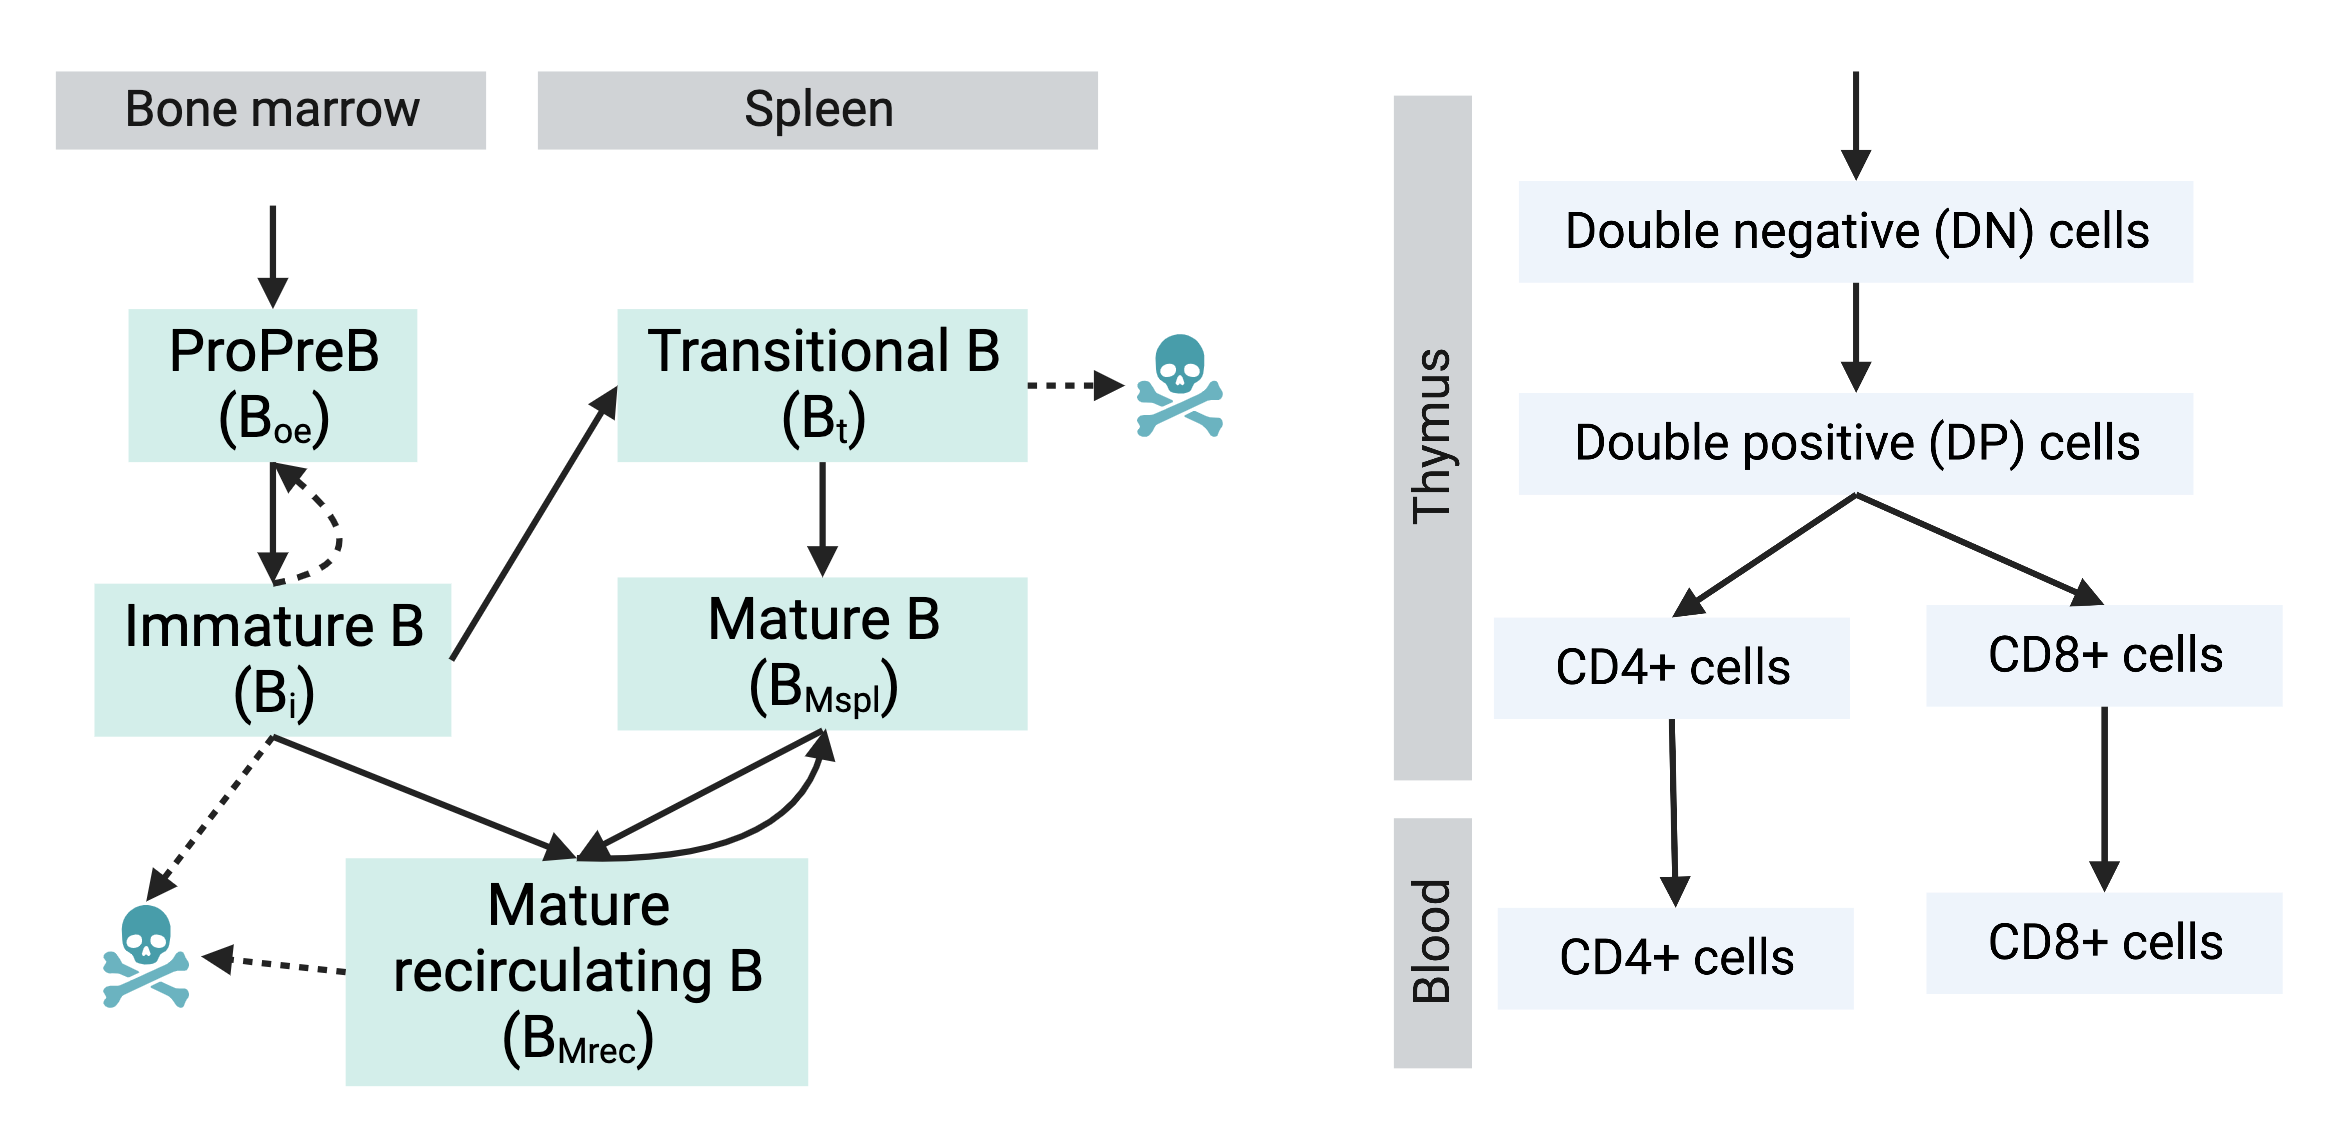
\includegraphics[width=\textwidth]{../img/Diagram_B_T.png}
\end{minipage}

The steady state of this model simulation compared well with mouse physiological data reported in literature. 
Furthermore, we demonstrate the model can predict the reconsititution dynamics of RBC, B cells, and T cells after HSC transplant in mouse published in Busch et al., Nature. 2015.  

\begin{minipage}[ht]{0.42\linewidth}
\begin{center}
\begin{tabular}{ c c c }
Cell type & Simulated & Reference \\ 
\hline
MPP & 60k & 75k-92k \\  
CMP & 2M & 755k- 3M  \\
GMP & 757k & 1M  \\  
GM & 8.4k/uL & 1.95-12.01k/uL \\  
RET & 498k/uL & 200 - 500k/uL   \\    
RBC & 9.9M/uL & 10.2M/uL   \\ 
blood Hb & 13.2g/dL & 13.6 - 16.4g/dL   \\ 
Hb in RBC & 261g/L & 270-330g/L  \\ 
lymphocyte & 1.8k/uL & 0.12 - 24k/uL  \\ 
\hline
\end{tabular}
\end{center}
\end{minipage}
\hspace{0.2cm}
\begin{minipage}[ht]{0.5\linewidth}
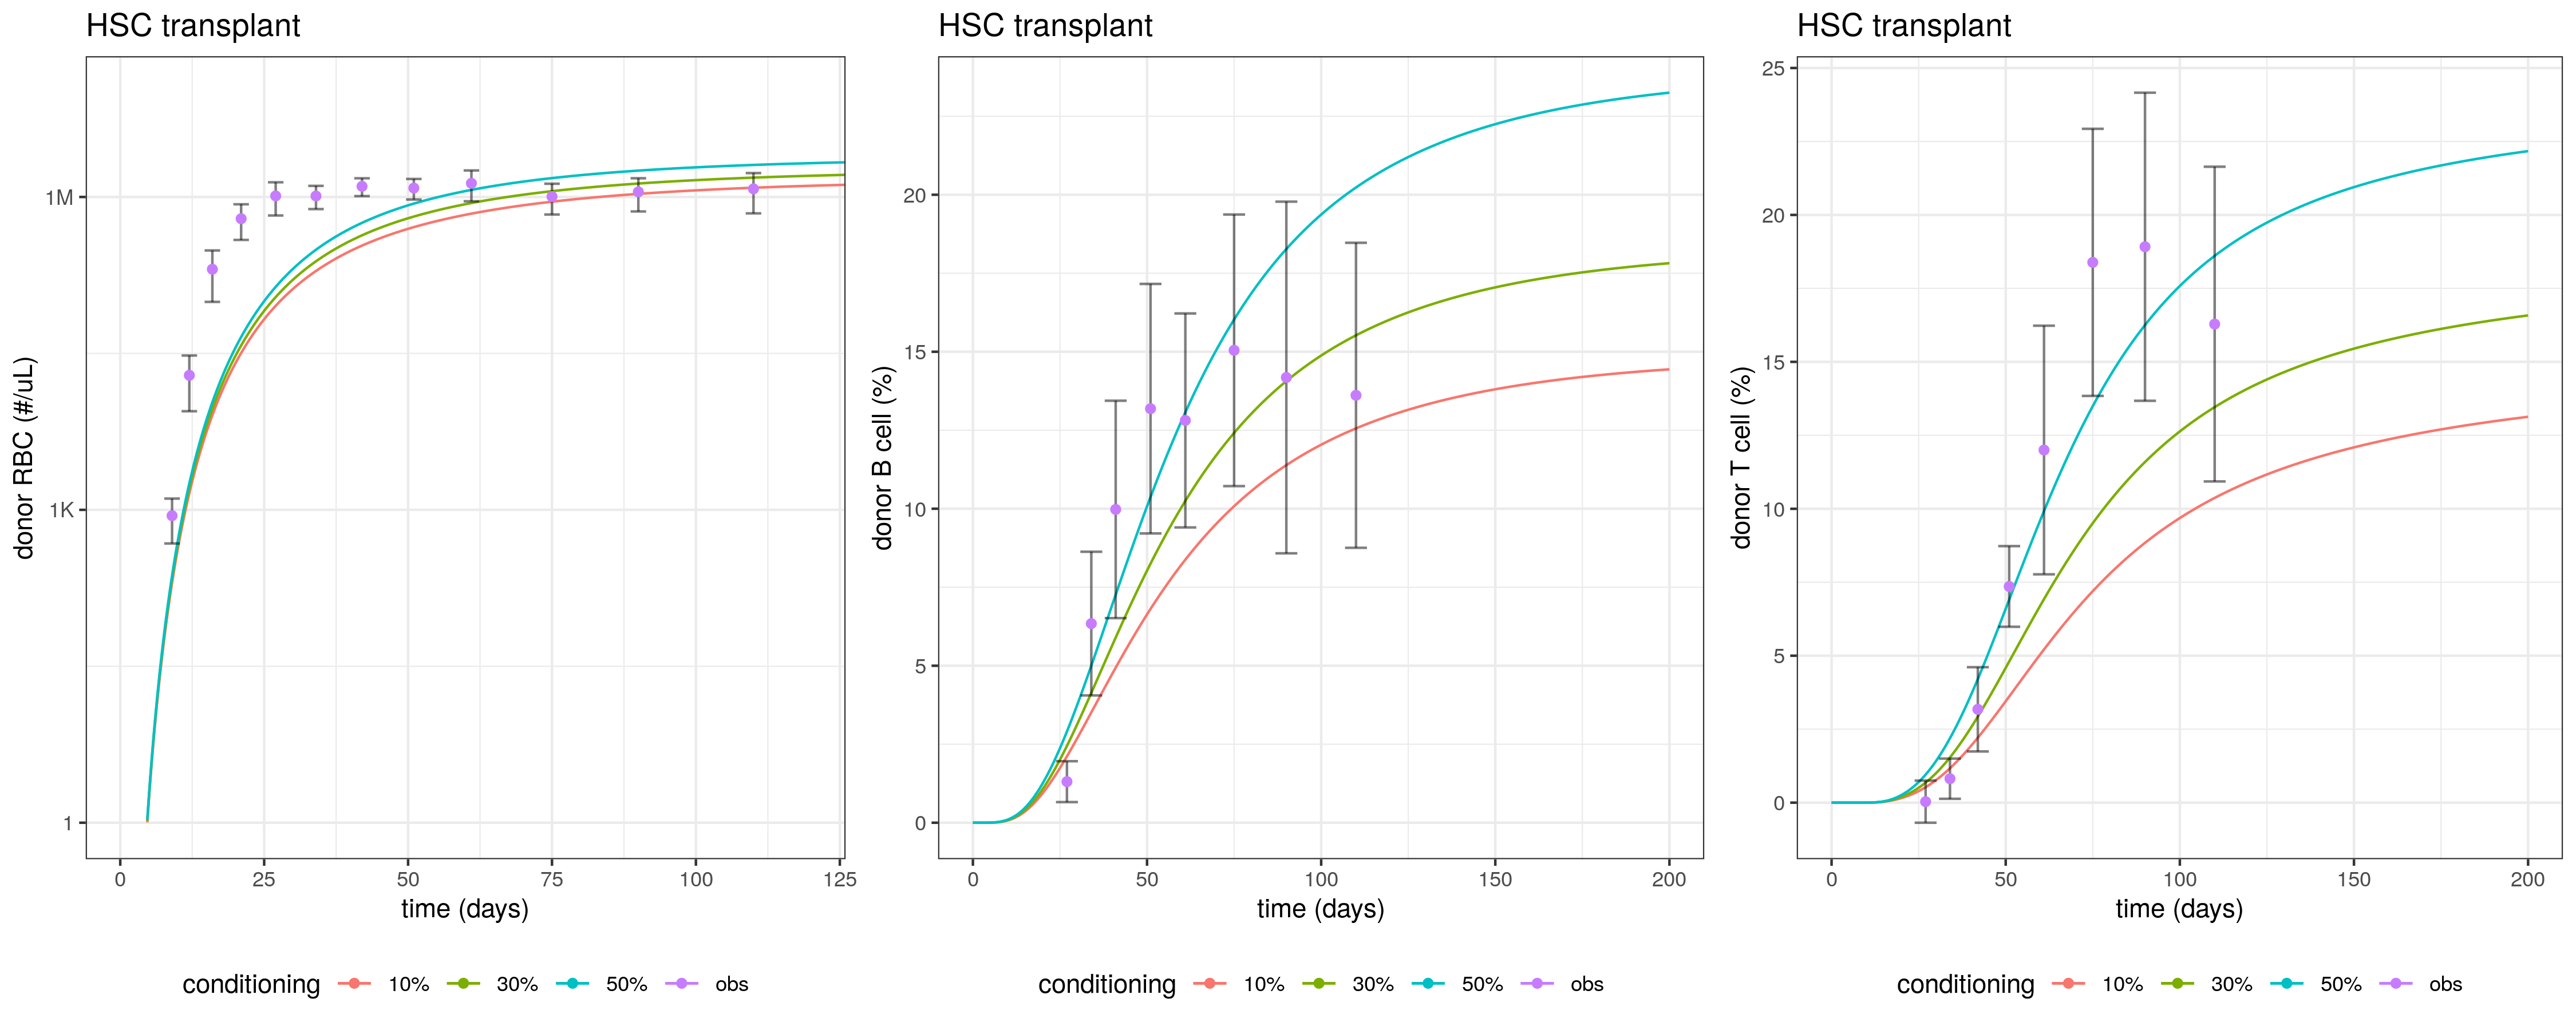
\includegraphics[width=\textwidth]{../img/mouse_RBC_T_B_HSCT.png}
\end{minipage}

Furthermore, the model was adapted to predict the ex-vivo gene therapy result on young mouse model with adenosine deaminase deficiency severe combined immunodeficiency (ADA-SCID). 
The model was adjusted to be more lymphoid-based (Young et al., J Exp Med. 2016), higher DP death rate (Whitmore and Gasper et al., Front Immunol., 2016), and higher mature B cell death rate in spleen and in blood (Whitmore and Gasper et al., Front Immunol., 2016, Blackburn and Kellems et al., Adv Immunol., 2005).
Assuming the radiation conditioning of Ada -/- mice resulted in 30\% loss of all dividing/ differentiating progenitors in the bone marrow, and 80\% loss in thymus, our model produce simulation results that is somewhat comparable to what was reported in Carbonaro et al., Blood., 2012. 


\begin{minipage}[b]{0.55\linewidth}
\centering
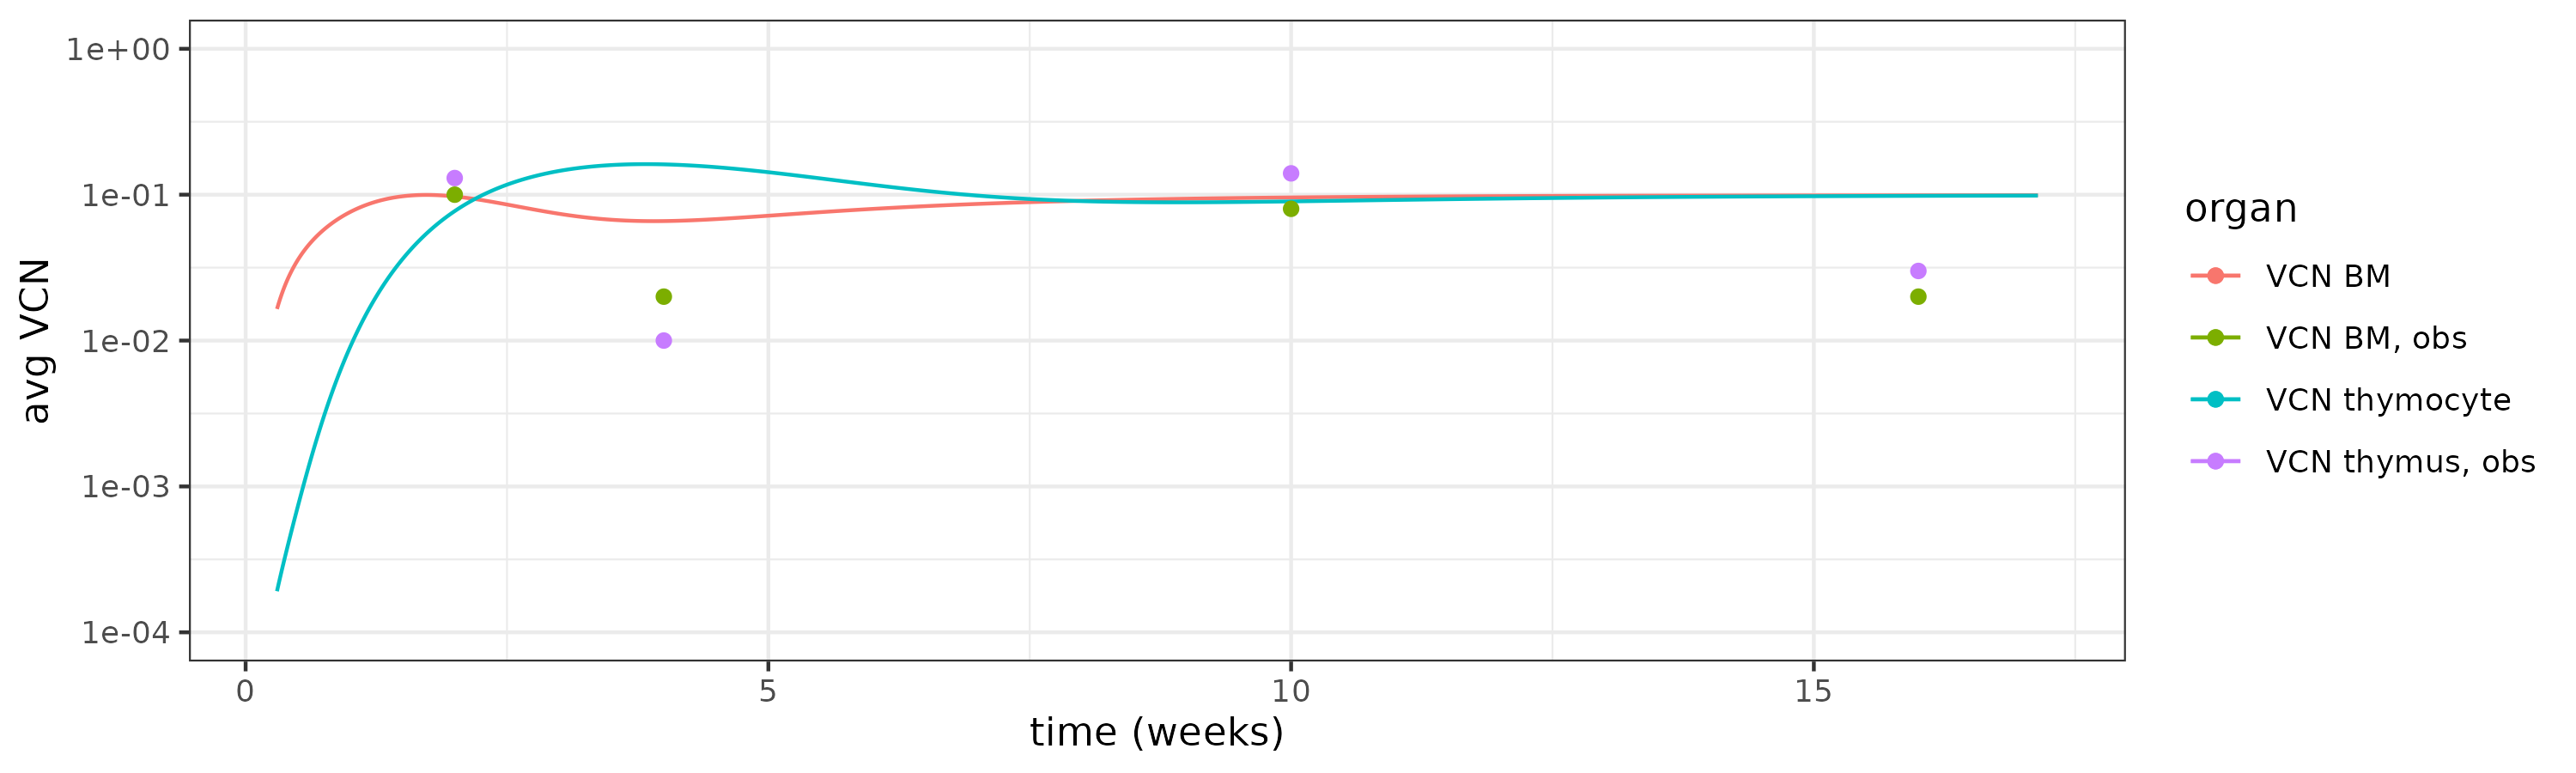
\includegraphics[width= 0.8 \textwidth]{../img/mouse_adascidgtsimul.png}
\end{minipage}
\hspace{0.5cm}
\begin{minipage}[b]{0.4\linewidth}
\centering
\end{minipage}
	



The integrated HSC differentiation model for human can be summarized by the figure follow. Briefly, the model was scaled from mouse to human and incorporated naive T cell dynamics in lymph nodes (LN) and peripheral tissues from [4].  


\begin{minipage}[b]{0.55\linewidth}
\centering
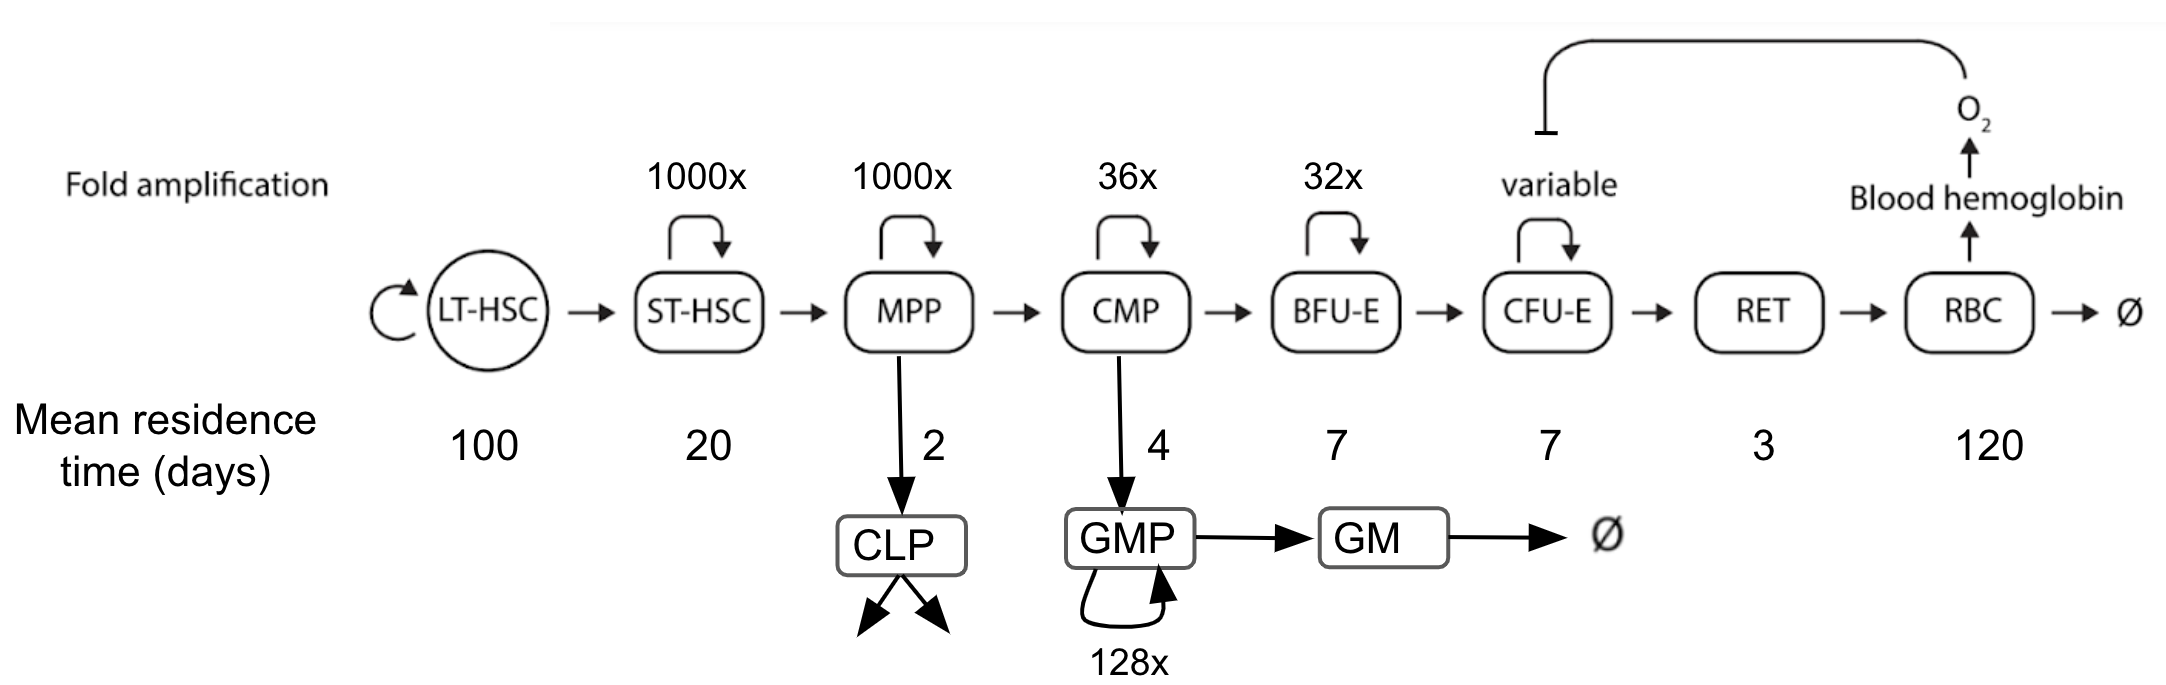
\includegraphics[width=\textwidth]{../img/human_full_structure.png}
\end{minipage}
\hspace{0.5cm}
\begin{minipage}[b]{0.4\linewidth}
\centering
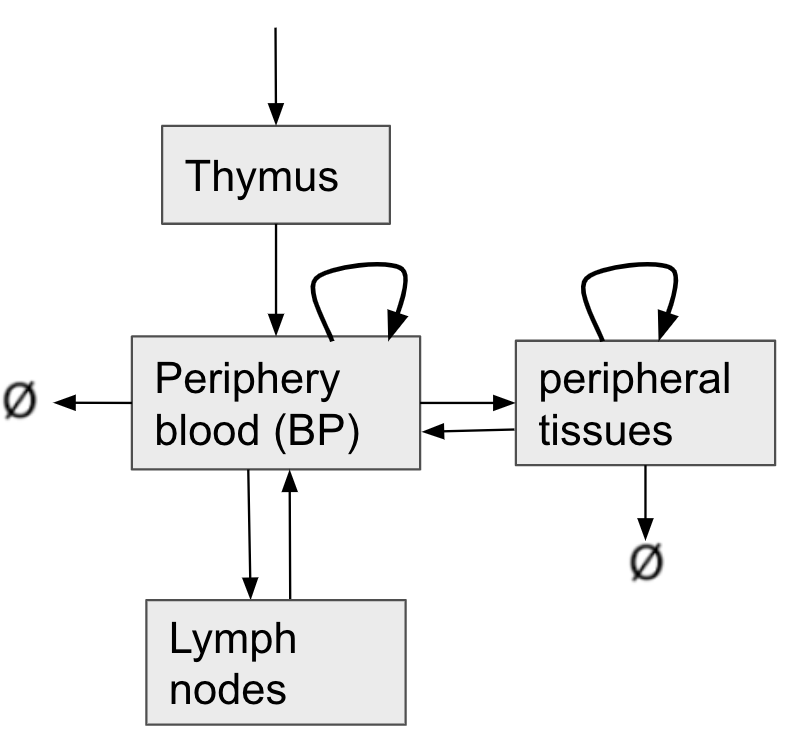
\includegraphics[width=\textwidth]{../img/human_naiveT.png}
\end{minipage}


}




%%%%%%%%%%%%%%%%%%%%%%%%%%%%%%%%%%%%%%%%%%%%%%%%%%%%%%%%%%%%%%%%%%%%%%%%%%%%%%%%


\headerbox{Conclusion}{name=conclusion,span=2,column=1,below=results}{
\footnotesize
Our work has resulted in a more comprehensive representation of mammalian hematopoietic stem cell development than previous partial efforts. Our integrated model is based on physiological understanding and validated with both mouse and human data. The models are implemented in both R and Julia, and the code will be available on GitHub. We believe this integrated model provides a versatile platform for predicting cell reconstitution after HSC transplant or ex-vivo gene therapy. 

}

\end{poster}
\end{document}
